\documentclass[../../main.tex]{subfiles}
\graphicspath{{\subfix{../../images/}}}

\begin{document}

\subsection{Warstwa użytkownika - frontend}
    \subsubsection{Struktura plików}
        Warstwa użytkownika została zaimplementowana przy pomocy frameworku Angular\cite{angular} opartego o język TypeScript (TS). Strukturę plików przedstawia Rysunek \ref{fig:frontend-repo-structure}.

        \begin{figure}[ht!]
            \begin{subfigure}{.5\textwidth}
                \centering
                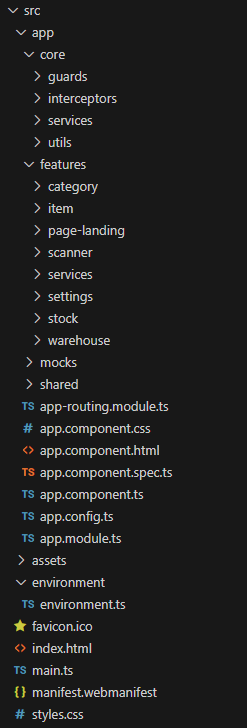
\includegraphics[height=0.4\pdfpageheight]{images/front-repo-structure.png}
                \caption{Ogólna struktura plików}
                \label{fig:front-repo-structure-general}
            \end{subfigure}
            \begin{subfigure}{.5\textwidth}
                \centering
                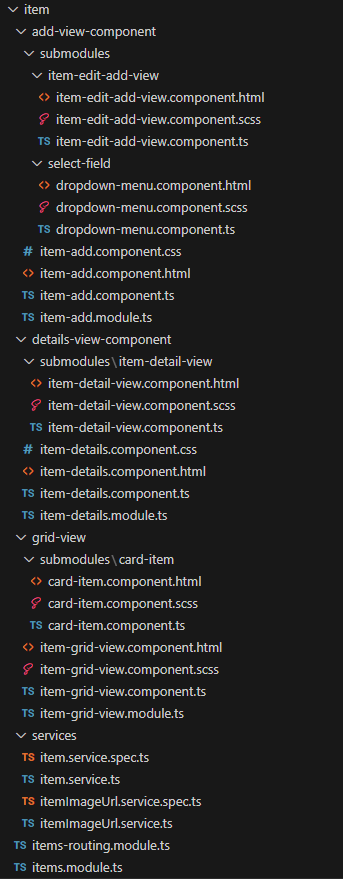
\includegraphics[height=0.4\pdfpageheight]{images/frontend-repo-structure-feature.png}
                \caption{Dokładna struktura jednego z komponentów}
                \label{fig:front-repo-structure-feature}
            \end{subfigure}
            \caption{Struktura plików frontendu}
            \label{fig:frontend-repo-structure}
        \end{figure}
    
        Aplikacja jest tworzona przy pomocy komponentów. Każdy komponent składa się ze skryptu TS, pliku stylu SCSS oraz pliku układu HTML. Dodatkowo niektóre komponenty korzystają z serwisów napisanych w języku TypeScript. Komponenty graficzne zazwyczaj mogą być wykorzystywane wiele razy i są one umieszczone w folderze \emph{shared}. Komponenty jednokrotne są umieszczone w folderze features i zawierają one kokretne implementacje poszczególnych widoków.
    \subsubsection{Widoki}
        % todo
    \subsubsection{Routing}
        % todo
    \subsubsection{Testy}
        % todo
    \subsubsection{Konteneryzacja - Docker}
        % todo

\end{document}